\chapter{Introduction}
\label{chap:intro}

\graphicspath{{../../assets/images/1/}}

The field of \ac{GIS} commits itself to the betterment of collecting, processing, storing, and viewing geodata. 
By doing so, it offers the world priceless information about the land we build on, the seas we traverse, the air we breath, and the climates we inhabit. 
This information is foundational for many applications, including environmental modelling, infrastructure, urban planning, governance, navigation, the military, and agriculture.   
As such, the field of \ac{GIS} is continuously looking for new ways to provide these fields and industries with both the data and tools they need to succeed. 

\subsection*{Problem Statement and Goal}

\begin{figure}
  \centering
  \begin{subfigure}[b]{\linewidth}
    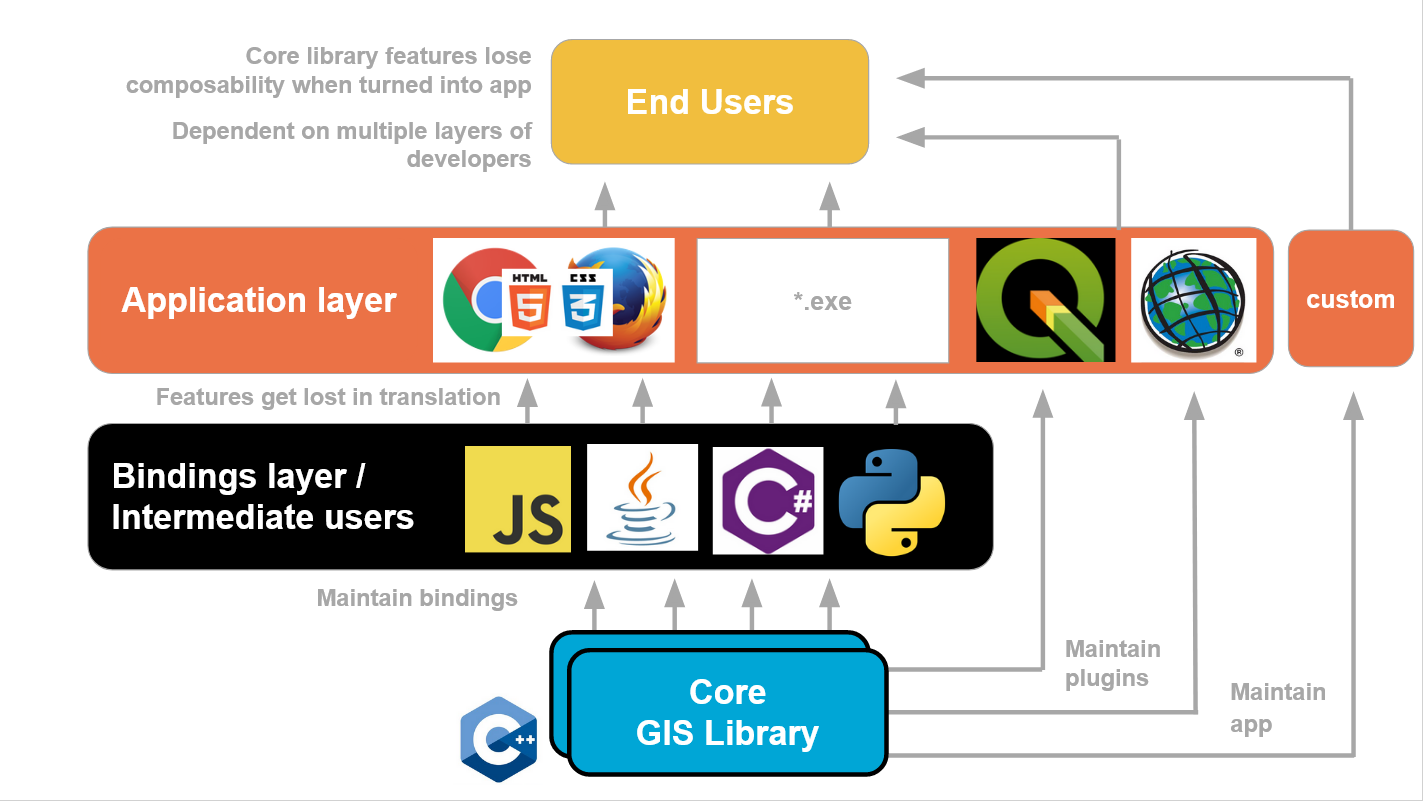
\includegraphics[width=\linewidth]{layers.png}
  \end{subfigure}%
  \caption{The layers of indirection between end users and core GIS functions}
  \label{fig:problem-statement}
\end{figure}

\begin{figure}
  \centering
  \begin{subfigure}[b]{0.40\linewidth}
  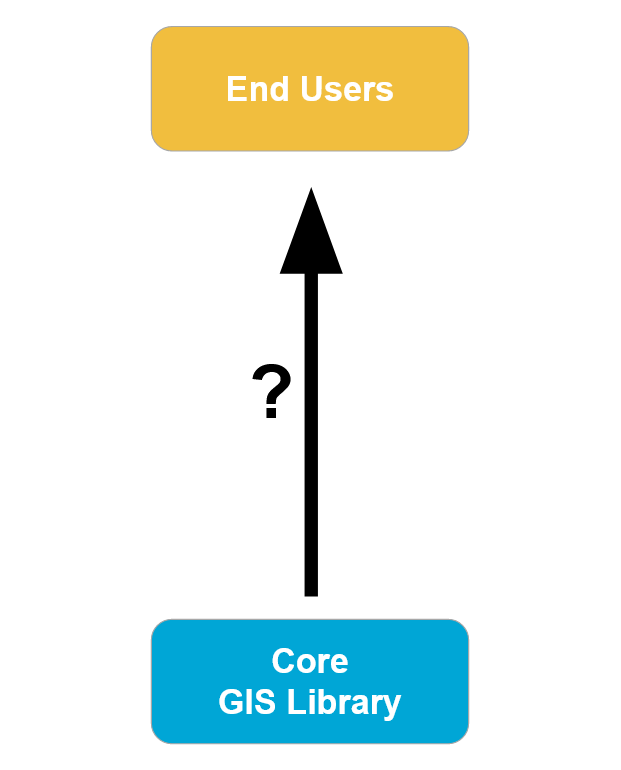
\includegraphics[width=\linewidth]{layers-simple.png}
  \end{subfigure}%
  \caption{The goal: More direct access}
  \label{fig:goal}
\end{figure}

This thesis concerns itself with the latter: Providing tools. 
The problem this study seeks to address, is that the core transformation and analysis tools found in certain \ac{GIS} software libraries, are normally not directly accessible by practitioners in the fields mentioned above: governance, infrastructure, urban planning, etc.
A small number of native software Libraries, like CGAL or GDAL \citep*{fabri_cgal_2009,dohler_gdal_2022}, play a foundational role in many \ac{GIS} tools. 
However, end users with a profession different than software developer, are often unable to directly access these libraries. 
The tools can only be used indirectly, and only when a software developer has incorporated these functionalities in an application. 
Similarly, if research leads to a new \ac{GIS} library, end users are at the mercy of a software developer implementing the functionalities of said library as a usable application, or as a plugin for an existing \ac{GIS} environment like QGIS \citep*{qgis_community_qgis_2022}.
Moreover, even if these capabilities are added to an application, the tools are almost always less feature rich, and non-composable: The output of one procedure cannot automatically be used as input for another. This leads to labor intensive procedures and repetitive workflows, as opposed to automated, re-usable procedures.
% Not taking advantage of the full potential of these libraries
At the same time, maintainers of a \ac{GIS} library often find themselves in the situation of having to maintain and synchronize a great number of bindings and plugins, which limits innovation (\reffig{fig:problem-statement}).

It is safe to say that the limited reach of these libraries translate to a reduced societal impact, and with it, the \ac{GIS} research these libraries are based upon.

% Not taking advantage of the full potential of these libraries 
% Not taking advantage of the full potential of 3DCMs applications due to lack of (good)
% maintenance is equivalent to discarding information already obtained. Considering
% the versatility of 3DCMs and how entangled cities are with society,  Furthermore, lim-
% itations in maintenance such as lack of managing tools by the organizations that
% possess the 3DCM, increases the administrating costs of a 3DCM. This often results
% into outsourcing —the biggest part of— its maintenance, by providing the neces-
% sary component-datasets to third parties. In some cases the solution for an updated
% 3DCM includes the (re)generation of completely new iterations of the model from
% scratch [Airaksinen et al., 2019], through, that a very small proportion of practitioners is able to perform.

The overarching goal of this study is to allow end-users more \textbf{direct} access to core transformation and analysis capabilities found in native \ac{GIS} libraries (\reffig{fig:goal}), in a format which allows \textbf{composability}.

The study attempts to meet this goal by studying two domains in the field of \ac{GIS}, and developing a possible solution from them.
The goal of \textbf{composability} is addressed by using the knowledge found within the field of \textbf{visual programming}.
The goal of \textbf{direct accessibility} is met by studying the field of \textbf{static web applications}.  
To make the research goals of this study more precise, these two domains must briefly be addressed.
% taking advantage 

% new relationship between GIS web UI's, and 

% \begin{note}
  
% VPL: Bridge between application and library
% - I want to focus on this particular reason for a VPL. 
%   - but, more reasons for using VPLs exist, such as end-user development (eud) (source)

% It is this particular aspect which sees significant usage in other applied CG fields, but not GIS.



% PROBLEM STATEMENT

% - VPLs are relatively unexplored within the field of GIS. 
%   - VPLs serve mostly as developer tools (ETL)
  
% - This thesis 
%    - provide capabilities of core geo-libraries directly to end-users.
%    - provide these capabilities in a composable way using a VPL. 
%    - provide customizable, composable UI.
%    - provide a way to scale this.

% - For this, a web-based, serverless VPL will be developed.

% + GIS VPL, 
 

% If we sum up these various considerationss


% \end{note}

% The web based geocomputation VPL is a novel development, and contains a multitude of unaddressed challenges.
% This study focusses on the particular problem of library portability. % and integration

% Successful geocomputation pipelines often relies on operations found in a select number of libraries. 
% Most major, industry-standard geocomputation libraries are native, C++-based libraries. 
% Examples of these are GDAL, PROJ, and GEOS. 
% However, A web based geocomputation VPL like the Mobius Modeller does not make use of these libraries, and usesJavaScript equivalents like Turf \citep{turf_contributors_turfjs_2022}.
% While it is possible to port a library like GDAL toJavaScript, guarantying that these two versions show the same behavior will be complex and time consuming. Additionally, managing duplicate libraries like this will slow down development, or create large version discrepancies \citep{ammann_maplibre-rs_2022}.

\subsection*{Composability: Visual Programming}

\begin{figure}
  \centering
  \graphicspath{{../../assets/images/background/geo-vpl/}}
  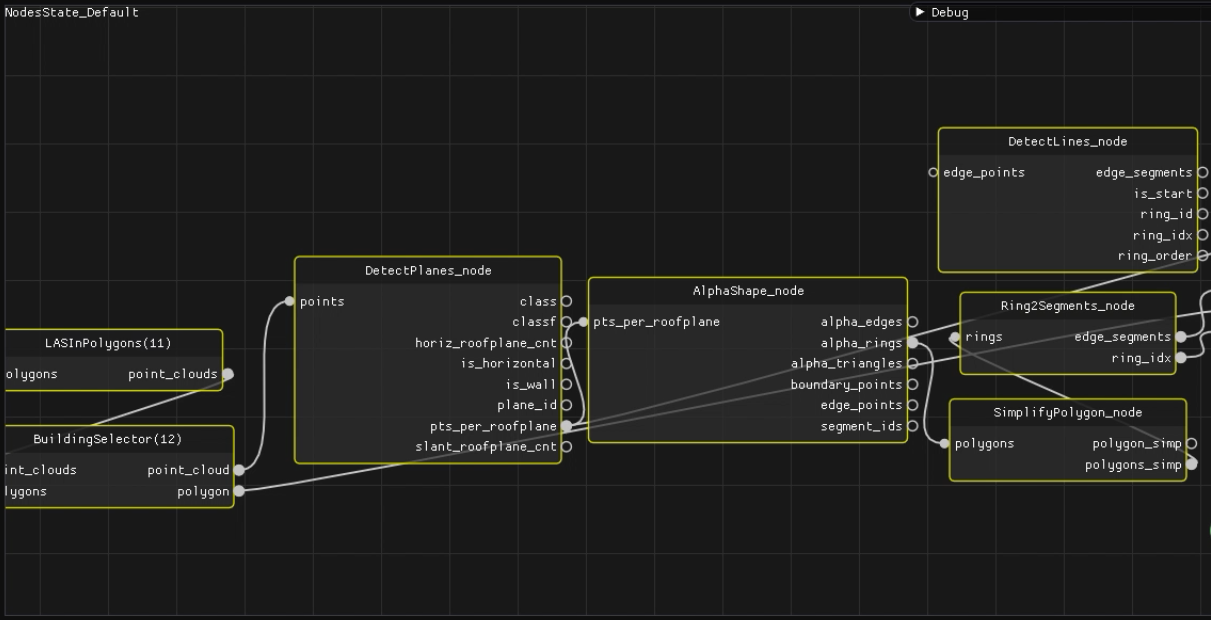
\includegraphics[width=\linewidth]{geoflow.png}
  \caption{Geoflow: An example of a graph-based VPL \citep{peters_geoflow_2019}}
  \label{fig:1:geoflow}
\end{figure}

A \ac{VPL} is a type of programming language represented by a \ac{GUI}, rather than a text-based source code.
A \ac{VPL} 'script' might take the shape of for example a graph (\reffig{fig:1:geoflow}), or a block-based instruction set.

The goal and purpose of a VPL can be framed in multiple ways. 
This study draws from the perspective presented in \citet{elliott_tangible_2007}, as it bears resemblance to the goal of this study.
\citet{elliott_tangible_2007} focusses on the discrepancies between software libraries, and software applications, and notes that in certain situations, properties of both libraries and applications are desired. 
Software libraries often contain expressive, re-usable functionalities, but do not provide a \ac{UI} of themselves, and must be turned into an application before utilization.
Software applications on the other hand, can offer a rich \ac{GUI}, but lose the ability to be re-composed into new software like libraries. Additionally, library functionalities presented through an applications are often reduced and less feature rich compared to the functionality of the library itself.
A VPL can be seen as an attempt to extract the best properties of both software libraries and applications. 
It can offer composability to applications, and \ac{GUI}s to libraries.
 
Because of these reasons, a VPL can be desirable format for a \ac{GIS} application.
Multiple examples exist, like FME \citep{safe-software_fme_2022}, Modelbuilder \citep*{esri_modelbuilder_2022} and Geoflow \citep{peters_geoflow_2019}.
However, if a VPL is meant to operate on geodata, it will have to attend to the nature of geodata. 
% application which both offers visualization and composability is 
% Two important characteristics of \ac{GIS} are the size and spatial nature of geodata.
The size of geodata makes scalable computation a necessity, and as such, GIS VPLs often contain tools to run these scripts on a server, without the \ac{GUI}. 
The spatial nature of geodata means that visualization is key in understanding its quality. 
Also, in most cases a visualization represents the end product of a \ac{GIS} process.
Both make it so GIS VPLs emphasize data visualization.  
Finally, \ac{GIS} Procedures sometimes require empirically defined parameters, which could be provided in a VPL using \ac{GUI} features like sliders. 

% This makes viewers an important component of the field.

% As such, the field often finds itself desiring solutions 
% or a \ac{GIS} operation
% Lastly, a VPL can aid with the parametrization of \ac{GIS} procedures. 
% Procedures like RANSAC take many 'magic parameters', which often need to be configured empirically, that is to say: "By trial and error". The Right UI can aid this.

% WHY GIS for VPL: 
% - a gis VPL requires attention to scalability. 

% ADDRESS THE QUESTIONS

% libraries 
% means to an end

% applications 
% the end (dead end)


% The split has drawbacks: 
% - Applications limit access to functionalities 
% - Applications are ususally not composable

% - Libraries have limited access and usage.
% - The medium affects

% The dream: 
% - unlimited access to functionality & composability, usability, and composability

% TODO ADD THIS TO RELATED WORKS SECTION 
% A VPL interface could also be valuable for different reasons. 

% constructing or editing a program in a visual way can be a faster process than using a textual method, even for the most experienced software developers \citep{green_usability_1996, kuhail_characterizing_2021}.
% Additionally, a \ac{VPL} allows for so-called End User Development \citep{kuhail_characterizing_2021}.
% A \ac{VPL} makes development more accessible to end users, as it allows practitioners to automate some processes and workflows like a software developer, but without needing a full background in software development \citep{benac_recent_2022}. 
% Finally, a VPL may even possess performance and reliability advantages over textual languages if it is implemented as a dataflow-type VPL \citep{sousa_dataflow_2012}. 

% These qualities are beneficial to geocomputation, and perhaps as a consequence, geocomputation by means of visual programming is not an uncommon phenomena in the field of \ac{GIS}.
% For example, Safe software's FME \citep{safe-software_fme_2022} is a popular \ac{VPL} among \ac{GIS} practitioners, arguably due to the way it simplifies the process of writing a \ac{ETL} pipeline. 
% Another example is McNeel's Grasshopper \citep{rutten_grasshopper_2012}, often used for small-scale spatial analyses, like solar irradiation or heating demands of a neighborhood \citep{sadeghipour_roudsari_ladybug_2013}. 




%%%%%%%%%%%%%%%%%%%%%%%%%%%%%%%%%%%%%%%%%%%%%%%%%%%%%%%%%%%%%%%%%%%%%%%%%%%%%%%

% \subsection*{Shortcoming: No true dataflow programming}

% The assumption that a geo-web-vpl should be implemented as a dataflow VPL is made because of the many advantageous qualities layed out in \refsec{sec:background:dataflow}. 
% Additionally, and perhaps consequently, all comparable VPLs analyzed in \refsec{sec:related-geovpl} were implemented as dataflow VPLs (Blender, houdini, Grasshopper, GeoFlow), the only exception being the Möbius Modeller.
% However, this meant that a new, web-based implementation had to be made, since no existing web-vpl concerned with geometry uses this model (that this study is aware of).



\subsection*{Direct access: Static web applications}

The maps and analysis tools used to share geo-information often take the form of web applications.  
A web applications offer distribution advantages over native applications \citep{kuhail_characterizing_2021, panidi_hybrid_2015}. 
It allows the same source code to be used across different platforms without alteration, including windows, mac, linux, and mobile devices. 
Moreover, web applications do not need to be installed, and can often be directly accessed using a link. 

Two major developments have occurred with great relevance to web GIS applications.

The first development concerns static file hosting.
Various geodata formats are increasingly becoming available as singular, statically hosted files, 
as opposed to the active \ac{OGC} web services which query databases, and use dynamic routing \citep{open_geospatial_consortium_web_2015}.
Examples of these static formats are the Cloud Optimized GeoTiff \citep{sarago_cloud_2021}, and the COPC file format \citep{bell_cloud_2021}. 
Static file hosting is orders of magnitude more cheap in terms of performance and literal cloud-host pricing, and scales more easily to accommodate high amounts of web requests \citep{sarago_cloud_2021}.

The second development is the introduction and adoption of the WebAssembly language \citep{haas_bringing_2017}. 
\ac{wasm} is a binary compilation target meant for a virtual runtime. 
\ac{wasm} binaries can be run in any environment and language, as long as such a runtime is implemented. 
Such a runtime has been added to all major web browsers since late 2019 \citep{w3c_world_2019}. 
Among many purposes, it offers a method to run native software as (part of) a web application. 
WebAssembly partially mitigates the need for web-based, JavaScript alternatives of native software applications and libraries. 
An Example of this is how \citet{ammann_maplibre-rs_2022} built one map viewer, which was both able to serve as a native and web application.

% Impact: Webassembly allows an expanded definition of 'cross-platform libraries' [mapbox.rs]
%   - This is benefitial for the same reason as traditional cross-platform arguments: 
%     - no duplicate libraries, no burden of synchronizing functionality across multiple libraries   

Both these developments taken together leads to a \\
paradigm shift which is important to recognize.
With both used in conjunction, \ac{GIS} applications can be conceived which use no active servers at all: Statically hosted websites, which can still be feature-complete as regular \ac{GIS} applications.

% This leads to valuable new options for web \ac{GIS}, such as making browser-based geocomputation more viable \cite{hamilton_client-side_2014, panidi_hybrid_2015, kulawiak_analysis_2019}. 

% A current, regular GIS web application would likely utilize OGC standardized web services like WMS, WFS, WMTS, or WPS, \citep{open_geospatial_consortium_web_2015} to access or process all requested geodata. 
% However, statically hosted geodata might mitigate the need for WMS, WFS and WMTS, and WebAssembly could replace certain WPS and backend geocomputation services.  


% more autonomous: Can operate more independently from its back-end counterpart.

% Serverless web applications
% This leads static hosting to be a cheaper alternative to active servers.


% This study seeks to contribute to serverless GIS web applications.
% In particular, this study wishes to explore if a new type of application is possible because of these developments. 
% A web application which is able to directly utilize core transformation and analysis capabilities found in native geo-libraries. 
% the capabilities of such an application: A serverless, 
% allows web applications to 
% Together, these technologies could be used to offer geodata and the means to process them 
% asks \ac{GIS} researchers to rethink our current models of GIS web applications. 
% - WebAssembly can be used to bring almost any transformation and analysis tool to a web application. 
% also offer the opportunity of geocomputation in the browser, instead of native
%   -> serverless geocomputation: geocomputation without any active server. 

% <!-- 
% (-> Benefits reproducibility & open science:)
%     (- Software developed is not only open source, but directly usable.)
%     (- Developers are forced to address the openness of data used.) -->




% -> This enables serving more people while using less computational resources on the backend. 
% , this might allow for a new type of GIS web application, 
% one which can operate 'serverless': Meaning no active server is required for using the web application. 

\subsection*{Taken Together}

Given both phenomena together, it becomes clear that the interface of a \ac{VPL} might present a solution to the problem of composability, for it allows both automation and a rich \ac{GUI} within one application. 
In addition, a combination of WebAssembly and a static web application could allow for direct access and execution of native \ac{GIS} libraries without installation, using statically hosted geodata as its data source. 
However, if a VPL wishes to 'qualify' as a GIS VPL, it needs to:
\begin{enumerate}
  \item be scalable to handle sizable datasets.
  \item provide a rich \ac{GUI}, capable of visualizing geodata, and quickly exploring different parametrization of various procedures.
\end{enumerate}

\section{Research Objective}


The goal of this study is to allow \ac{GIS} practitioners without a background in software development, to access the full potential of core transformation and analysis capabilities found in native \ac{GIS} libraries.

The study attempts to meet this goal by designing and implementing a novel \\ method based on the fields of visual programming, and static web applications. 
This method is thereafter used to load various \ac{GIS} libraries, and used in demo applications, after which an assessment can be made on its quality and the extent of its achieved functionalities. 
The study concludes by addressing if the method meets its overarching goal.

% The prior works on static geo-web applications and \ac{GIS} \ac{VPL}s indicate that a strong theoretical framework is in place.
% But, and this is especially evident in the prior studies regarding Browser-based geocomputation, the practical implementation of these theories were only partially successful, and limited in scope. 
% This necessitates a practical approach in response. 

While VPLs and even Web-based VPLs have been studied before in the field of \ac{GIS}, the focus on direct utilization of native \ac{GIS} libraries on the web, combined with bringing those in direct contact with various \ac{GUI} elements, all without resorting to active web servers, is a combination unique to this study, at least to the best of the authors knowledge at this point in time. 
A comparative study on \ac{VPL}s found in the field of \ac{GIS}, Computer graphics, the web, and generic VPLs, is  performed to ensure this.
Additionally, assessment criteria are used to ensure this remains true after having performed the study.
% Certain implementation details also offer a novel take on \ac{VPL}s as a whole.

The overall design of the prototype outlined contains a number of technical challenges.
The compilation of native libraries to Webassembly is known to contain drawbacks, and achieving scalability with a VPL requires exploration of novel methods. 
Therefore, seeking and analyzing solutions to these challenges is required to making this prototype meet the goals of the design mentioned. 

% more direct access in a format which allows composability.
% The study attempts to meet this goal by designing a visual programming language, implemented as a static web application.
% This study
% VPL for web-based, serverless geocomputation has not been tried yet. 
% This study seeks to improve the state of browser-based geocomputation VPLs.
% This is done by studying a possible solution to the library portability problem found in existing browser-based geocomputation VPLs.
% The study poses that the library portability problem can only be overcome if native geocomputation libraries are able to be properly compiled, loaded and utilized in a browser-based dataflow-VPL format. 
% There are multitude of technical challenges present within each one of these steps, and in between these steps. 
% Seeking and analyzing solutions to these challenges is the focal point of this study. 


\section{Research Questions}
The objectives outlined above lead to the following main and supporting research questions:  
\begin{itemize}[ ]
  \item \myNewMainRQ
\end{itemize}

\subsection*{Supporting Questions}

\begin{itemize}[-]
\item \myNewSubRQOne
\item \myNewSubRQTwo
\item \myNewSubRQThree
\item \myNewSubRQFour
\item \myNewSubRQFive
\end{itemize}

\subsection*{Assessment}
In order to proof if the proposed method is viable or not, tests will be performed primarily based upon feature completeness.
Within the context of this study, whether or not a feature was able to be implemented given the constraints of the method (web based, visual programming), was often deemed a more insightful indicator compared to measuring aspects like performance and memory footprint.
The thesis sets out to proof or disproof technical viability. 
Future research is required to test \emph{How} viable it might be compared to other, comparable methods.

% Such subjects are only relevant in comparison to similar methods, and this study in particular aims to develop a novel method, 
% which by definition should be differ to existing methods. 

% It must be tested if all required features are able to be

% It is important to recognize that the above research questions do not cover subjects like performance, accuracy, memory footprint, etc. 
% However, it does cover accessibility, and composability. 

% To adequately assess these concepts, 




% \begin{note}
% TODO: diagram: 4 research questions -> four possible barriers of geocomputation
% \end{note}

% \begin{note}
% TODO: diagram: show the 'locations' of the four research questions ( client / server / native, etc.)
% \end{note}

% \subsection*{Nature}
% The methodology of this study can be characterized as practical as opposed to theoretical, 
% % wholistic instead of specific, 
% and iterative compared to linear. 
% The prior works on browser-based geocomputation and geo-vpls indicate that a strong theoretical framework for a \ac{geo-web-vpl} is in place (Source). 
% But, and this is especially evident in the prior studies regarding Browser-based geocomputation, the practical implementation of these theories were only partially successful, and limited in scope. 
% This necessitates a practical approach in response. 
% And, due to the investigative nature of this study, the methodology requires to iterate upon itself, instead of following a singular, linear path. 

% MIGHT NOW WANT TO KEEP THIS IN HERE
% ...
% % Theorie: is er maar je geloofde het niet
% % praktische implementatie om de Throerie weerleggen
% The prior works on browser-based geoprocessing indicate that a theoretical framework for browser-based geoprocessing VPL is in place. 
% But, and this is especially evident in the studies regarding client-side geoprocessing, the practical implementation of these theories

% Choices: 
% - practical > theoretical : Literature study indicates enough theoretical soundness, but lots of practical questions remaining. We wish to  immediate pick up where these studies have left, and therefore we choose the direct, practical study of designing and implementing a prototype application. 
% - wholistic > specific    : Research in one sub-domain could have been more exhaustive in one of the specific sub-studies, instead of covering the full scope it does now. However, This would have been incomplete. What we do now is cover the full pipeline of using a geocomputation library: from creation to web export, to web import, to web utilization. by doing this, we can identify issues caused in one of these
% - iterative > linear      : Given this vast scope, many questions can come up from different angles. The study has to be dynamic to adapt to these demands. 

\section{Scope}
The scope of this thesis is bounded in the following ways: 

\subsection*{Only frontend geocomputation}

There is a nuance between 'web-based geocomputation' and 'browser-based geocomputation'. 
'Web' can refer to both frontend and backend computation methods, 'browser' refers purely to frontend computations. 
This study focusses on browser-based geocomputation, and as such, excludes any \emph {backend} based geocomputation.

Adding backend-based geocomputation to a web VPL would be an excellent 
follow-up investigation to this study, following in the footsteps of studies like \cite{panidi_hybrid_2015}.

\subsection*{No user testing} % 

The introduction mentions \emph{accessibility} as a motivator, which is a subjective concept.
However, user testing is not part of this study, due to scope limitations. 

To solve this, this study assesses accessibility without regarding subjective, psychological accessibility aspects: \emph{"does x feel nice to use?"}.
Instead, an accessibility assessment is made by only regarding feature completeness: \emph{"Is is possible to do X with Y?"}.
Moreover, certain presuppositions are made.
It is safe to assume that a web application is more accessible than a native application, for it mitigates installation needs. 
Additionally, a VPL is assumed to be more accessible than normal programming.
This last aspect is safe to assume based on the findings of \citet{kuhail_characterizing_2021}, stating that based on 30 independent studies on the accessibility of VPLs, VPLs are generally considered more accessible than their textual counterparts.
These studies involved user tests with professional programmers, amateur programmers, and non-programmers alike. 

Thus, these reasons together are why this study believes an adequate assessment can be made without user testing. 
Nevertheless, a follow up study to reinforce or revoke these results would be valuable.

% While accessibility and usability are motivations for this study, and while accessibility will be analyzed to a limited extent, 

% no claims will be made that this method of geocomputation is \emph{more} usable as opposed to existing geocomputation methods. 

% This research attempts to solve the practical problem of library portability. 
% We must therefore access if a library can be \emph{used} in a VPL context. 



% If it turns out that library portability is viable enough technically, future research will be needed to definitively proof \emph{how} usable VPL usage of a library is compared to all other existing methods. 
% Similarly, a survey analyzing how users experience browser-based geocomputation in comparison to native geocomputation is also not part of this particular study.  

% This distinction is made, because browser-based, VPL-based geocomputation is too new of a method to make a balanced comparison against any other methods. 
% Native environments like QGIS, FME or ArcGIS simply have a twenty year lead in research and development. 

% This paper seeks to first close this gap, limiting itself to overcoming the technical and design boundaries in the pursuit of practical client-side geocomputation.

% While the research restrains itself from empirically measuring an aspect as nebulous as 'accessibility', it does demonstrate ...

% It is my goal to introduce this as a new geocomputation option, and to name the advantages and disadvantages we can be sure of. An actual comparison of client-side vs native geocomputation is something different. 

\subsection*{Only WebAssembly-based containerization}

This thesis examines a WebAssembly-based approach to containerization and distribution of geocomputation functionalities. 
Containerization using Docker is also possible for server-side applications, but is not (easily) usable within a browser. 
For this reason, Docker-based containerization is left out of this studies' examination. 
And to clarify: Docker and WebAssembly are not mutually exclusive models, and could be used in conjunction on servers or native environments. 

% \subsection*{Mostly Point Cloud/ DTM focussed geocomputation}

% The scope of 'geocomputation' also needs to be concentrated, as it is a sizable phenomenon.
% The term is generally used to cover all operations on any type of geodata, from rasters, tabular datasets, highly structured datasets such as the CityJSON or IndoorGML, and point clouds. 
% Due to time limitations, we are forced to focus on particular type of geocomputation.
% 3D-based geocomputation is chosen, with a particular focus on pointclouds and DTMs. 
% The hypothesis is that these types of data may fit the small-scale geocomputation of a VPL well due to the local optimality quality of many DTM procedures (Such as the \ac{DT}). 

% \subsection*{Assumption: a 'Geocomputation-VPL' is a Geometry VPL able to handle geodata}
% For the scope of this thesis, we assume a VPL for geocomputation is practically the same as a VPL for generic geometry processing.
% Examples of "Geometry VPLs" are Blender's Geometry Nodes, Houdini, and Grasshopper.
% More on this in chapter \refsec{sec:related-geovpl}.

% A Geocomputation VPL differs only in the fact that it supports additional geodata types, and offers functionalities specific to processing those types.  
% This assumption is safe to make since a geocomputation VPL will \emph{at the very least} require the same features as a 'normal' geometry VPL, due to their common dependency on the field of computer graphics and computational geometry.

% Still, in reality, a lot of differences and nuances exist between the field of geocomputation and the field of procedural modelling. 
% However, due to time limitations, these concerns are left to future research.
% these concerns will only be picked up at the final discussion, found at \refsec{sec:discussion}.
 
\subsection*{Only GIS libraries written in C++ \& Rust}

The study limits itself to native libraries written in C / C++ and Rust. 
C++ was chosen, since almost all relevant GIS libraries are written in C or C++, like GDAL \citep{dohler_gdal_2022}. 
Rust was chosen, for its extensive WebAssembly support. 
It also appears to be the most popular language for writing WebAssembly \citep{eberhardt_state_2022}.
It contains a number of relevant GIS libraries, but not to the same extent as C / C++.

% \subsection*{Only core browser features}
% Lastly, the implementation of the prototype geocomputation VPL will limit itself to core browser features, keeping dependencies at a minimum, in an attempt to generalize the results of the study.
% If the study would use specific web frameworks and technologies to solve key issues, questions might arise if the results of the study counts in general for browser-based geocomputation or geocomputation VPLs, or if they only count in this specific scenario. 
% "Core browser features" is defined in \refsec{sec:method:base-vpl}.

\section{Reading Guide}
The remainder of this study is structured as follows:

\begin{itemize}[ ]
  \item \refchap{chap:background}, Background, provides an overview of the theoretical background that is used in the rest of this study.
  
  \item \refchap{chap:related}, Related Work, provides a review of studies comparable to this one.

  \item \refchap{chap:methodology}, Methodology, explains precisely in what way the research-questions will be answered.
  In addition, the main design decisions are described and justified in this part of the study.

  \item \refchap{chap:implementation}, Implementation, presents the implementation of the methodology.
  
  \item \refchap{chap:testing}, Testing, tests the results from this implementation in various ways described by the methodology.
  
  \item And finally, \refchap{chap:conclusion}: Conclusion \& Discussion, concludes to which extent the study was able to satisfy the main research question, and discusses unaddressed aspects of the thesis.
  It also includes the envisioned future works and a reflection on the quality of the study.

\end{itemize}